\documentclass{article}

%Package Part
\usepackage{relsize,setspace}  % used by latex(describe( ))
\usepackage{url}               % used in bibliography
\usepackage[superscript,nomove]{cite} % use if \cite is used and superscripts wanted
% Remove nomove if you want superscripts after punctuation in citations
\usepackage{lscape}            % for landscape mode tables
\textwidth 6.75in              % set dimensions before fancyhdr 
\textheight 9.25in
\topmargin -.875in
\oddsidemargin -.125in
\evensidemargin -.125in
\usepackage{fancyhdr}          % this and next line are for fancy headers/footers
\pagestyle{fancy}
\newcommand{\bc}{\begin{center}}  % abbreviate
\newcommand{\ec}{\end{center}}

\usepackage{Sweave}
\begin{document}

\Sconcordance{concordance:test.tex:test.Rnw:%
1 18 1 1 0 14 1 1 21 4 1 1 2 31 0 1 1 24 0 1 1 14 0 1 1 27 0 1 2 2 1 1 %
6 1 2 5 1 1 2 1 3 1 2 4 1 1 2 1 3 1 2 2 1 1 2 1 3 1 2 4 1 1 2 1 3 1 2 3 %
1 1 2 1 3 1 2 2 1 1 2 1 3 1 2 4 1 1 2 1 3 1 2 3 1 1 2 1 3 1 2 2 1 1 2 1 %
3 1 2 2 1}


%\SweaveOpts{width=6, height=4}


\title{Performance Analysis}
\author{}
\date{}

\setkeys{Gin}{width=1\textwidth}
\maketitle
%\tableofcontents


\section{Overview}
This documents go through performance of \verb|tech|. Simulation period is from 2006-01-03 09:00:00 to 2013-01-25 09:00:00. The portfolio is composed with Large Caps (which hedge by Equity Trading Team in 'H' securities). Data source is WiseFN.

\subsection{Tables}
% latex table generated in R 2.15.2 by xtable 1.7-0 package
% Tue Jan 29 16:59:12 2013
\begin{table}[ht]
\begin{center}
\caption{Calendar Returns}
\begin{tabular}{rrrrrrrrr}
  \hline
 & 2006 & 2007 & 2008 & 2009 & 2010 & 2011 & 2012 & 2013 \\ 
  \hline
1 & 0.00 & -7.50 & -34.00 & -3.00 & -4.10 & 3.00 & 6.70 & -1.60 \\ 
  2 & 1.00 & 5.90 & -0.20 & -12.90 & -1.30 & -12.40 & 1.90 &  \\ 
  3 & 0.80 & 2.60 & -2.10 & 10.20 & 3.00 & 9.30 & -1.80 &  \\ 
  4 & 4.10 & 8.50 & 2.50 & 11.80 & 2.50 & 4.20 & -0.80 &  \\ 
  5 & -16.30 & 14.40 & -0.70 & 0.80 & -1.70 & -6.30 & -4.10 &  \\ 
  6 & 26.30 & -1.50 & -8.80 & -5.30 & 4.70 & -4.80 & -2.60 &  \\ 
  7 & -1.40 & 8.30 & -10.40 & 8.10 & 2.10 & -0.50 & -1.80 &  \\ 
  8 & 3.80 & -9.70 & -8.20 & 0.40 & 2.80 & -31.10 & 2.80 &  \\ 
  9 & 0.10 & 5.90 & -11.70 & 1.60 & 8.70 & -4.50 & 0.40 &  \\ 
  10 & 2.20 & 15.50 & -31.10 & -9.00 & -2.70 & -2.60 & -0.90 &  \\ 
  11 & 4.30 & -10.10 & -6.30 & -5.30 & -1.30 & -7.00 & 0.20 &  \\ 
  12 & -2.20 & -3.90 & 4.20 & 6.90 & 5.40 & -7.90 & 2.70 &  \\ 
  X1 & 19.60 & 27.00 & -70.70 & 1.10 & 18.60 & -50.00 & 2.30 & -1.60 \\ 
  X2 & 1.30 & -0.40 & -92.50 & 62.30 & 18.60 & 2.40 & -9.20 & -3.00 \\ 
  X3 & 7.00 & 51.20 & -42.50 & 67.20 & 26.80 & -6.00 & -2.10 & -3.60 \\ 
  X4 & -1.30 & -3.20 & -58.10 & -7.20 & -5.10 & -32.40 & -6.60 & -2.40 \\ 
  best.bm & 14.60 & -2.00 & -49.90 & -34.10 & -4.70 & -41.70 & -9.80 & 2.10 \\ 
  best.worst & 4.10 & -24.90 & -52.90 & -46.70 & -15.10 & -50.90 & -5.20 & 1.70 \\ 
  KM1 & 4.70 & 31.40 & -37.40 & 51.10 & 22.90 & -11.70 & 11.90 & -3.70 \\ 
   \hline
\end{tabular}
\end{center}
\end{table}% latex table generated in R 2.15.2 by xtable 1.7-0 package
% Tue Jan 29 16:59:12 2013
\begin{table}[ht]
\begin{center}
\caption{Calendar Returns}
\begin{tabular}{rrrrrrrrr}
  \hline
 & 2006 & 2007 & 2008 & 2009 & 2010 & 2011 & 2012 & 2013 \\ 
  \hline
1 &  & -5.20 & -14.80 & 4.10 & -5.90 & 0.10 & 8.10 & -3.70 \\ 
  2 & -1.40 & 3.50 & 4.50 & -9.70 & -0.60 & -6.90 & 3.50 &  \\ 
  3 & -0.30 & 3.10 & 0.60 & 14.90 & 7.00 & 9.50 & 0.30 &  \\ 
  4 & 4.40 & 5.80 & 8.70 & 11.50 & 2.80 & 3.60 & -0.90 &  \\ 
  5 & -7.40 & 8.30 & 0.30 & 0.60 & -6.90 & -2.60 & -8.50 &  \\ 
  6 & -1.70 & 2.20 & -9.80 & 0.90 & 3.60 & -2.10 & 1.30 &  \\ 
  7 & 1.00 & 10.40 & -4.30 & 13.10 & 4.30 & 0.70 & 2.10 &  \\ 
  8 & 4.30 & -1.70 & -8.00 & 1.90 & -1.50 & -13.30 & -0.00 &  \\ 
  9 & 1.80 & 4.60 & -1.00 & 6.90 & 7.40 & -4.50 & 5.70 &  \\ 
  10 & -0.50 & 5.10 & -20.50 & -7.30 & -0.60 & 9.70 & -5.20 &  \\ 
  11 & 4.20 & -6.90 & -2.90 & -0.60 & 3.60 & -3.80 & 2.00 &  \\ 
  12 & 0.60 & -0.10 & 5.60 & 8.80 & 9.00 & -0.60 & 4.10 &  \\ 
  KM1 & 4.70 & 31.40 & -37.40 & 51.10 & 22.90 & -11.70 & 11.90 & -3.70 \\ 
   \hline
\end{tabular}
\end{center}
\end{table}% latex table generated in R 2.15.2 by xtable 1.7-0 package
% Tue Jan 29 16:59:17 2013
\begin{table}[ht]
\begin{center}
\caption{Annualized Returns}
\begin{tabular}{rrrrrrrr}
  \hline
 & X1 & X2 & X3 & X4 & best.bm & best.worst & KM1 \\ 
  \hline
Annualized Return & -0.15 & -0.18 & 0.08 & -0.18 & -0.21 & -0.31 & 0.05 \\ 
  Annualized Std Dev & 0.24 & 0.34 & 0.27 & 0.28 & 0.21 & 0.25 & 0.26 \\ 
  Annualized Sharpe (Rf=0\%) & -0.61 & -0.53 & 0.28 & -0.65 & -1.04 & -1.22 & 0.20 \\ 
   \hline
\end{tabular}
\end{center}
\end{table}% latex table generated in R 2.15.2 by xtable 1.7-0 package
% Tue Jan 29 16:59:17 2013
\begin{table}[ht]
\begin{center}
\caption{Statistics}
\begin{tabular}{rrrrrrrr}
  \hline
 & X1 & X2 & X3 & X4 & best.bm & best.worst & KM1 \\ 
  \hline
Observations & 1758.00 & 1758.00 & 1758.00 & 1758.00 & 1757.00 & 1758.00 & 1757.00 \\ 
  NAs & 0.00 & 0.00 & 0.00 & 0.00 & 1.00 & 0.00 & 1.00 \\ 
  Minimum & -0.10 & -0.58 & -0.11 & -0.11 & -0.10 & -0.12 & -0.10 \\ 
  Quartile 1 & -0.01 & -0.01 & -0.01 & -0.01 & -0.01 & -0.01 & -0.01 \\ 
  Median & 0.00 & 0.00 & 0.00 & 0.00 & -0.00 & -0.00 & 0.00 \\ 
  Arithmetic Mean & -0.00 & -0.00 & 0.00 & -0.00 & -0.00 & -0.00 & 0.00 \\ 
  Geometric Mean & -0.00 & -0.00 & 0.00 & -0.00 & -0.00 & -0.00 & 0.00 \\ 
  Quartile 3 & 0.01 & 0.01 & 0.01 & 0.01 & 0.00 & 0.01 & 0.01 \\ 
  Maximum & 0.15 & 0.08 & 0.12 & 0.12 & 0.13 & 0.13 & 0.10 \\ 
  SE Mean & 0.00 & 0.00 & 0.00 & 0.00 & 0.00 & 0.00 & 0.00 \\ 
  LCL Mean (0.95) & -0.00 & -0.00 & -0.00 & -0.00 & -0.00 & -0.00 & -0.00 \\ 
  UCL Mean (0.95) & 0.00 & 0.00 & 0.00 & 0.00 & -0.00 & -0.00 & 0.00 \\ 
  Variance & 0.00 & 0.00 & 0.00 & 0.00 & 0.00 & 0.00 & 0.00 \\ 
  Stdev & 0.02 & 0.02 & 0.02 & 0.02 & 0.01 & 0.02 & 0.02 \\ 
  Skewness & 0.31 & -11.24 & -0.20 & -0.15 & 0.62 & 0.11 & -0.24 \\ 
  Kurtosis & 11.17 & 286.78 & 5.48 & 6.93 & 17.82 & 9.91 & 4.96 \\ 
   \hline
\end{tabular}
\end{center}
\end{table}
\subsection{Distribution}

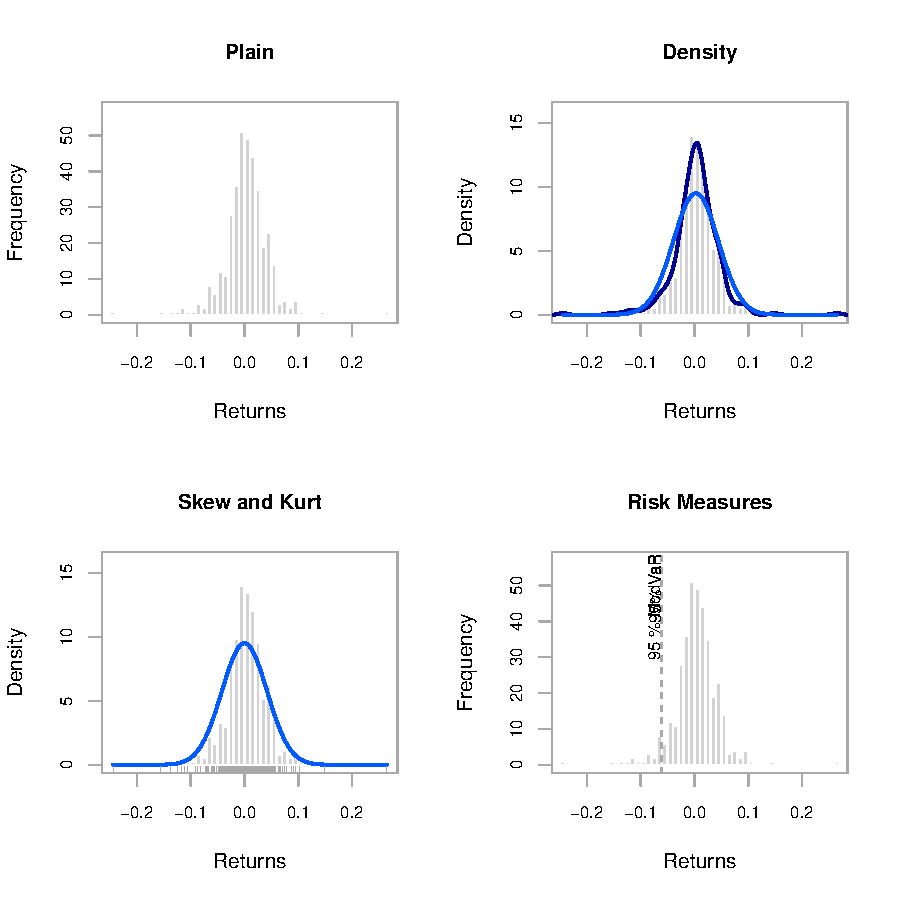
\includegraphics{graphics/plot-003}

\section{All yr Performance}
\setkeys{Gin}{width=0.5\textwidth}
%\begin{landscape}
\subsection{Returns}
\begin{tabular}{cc}
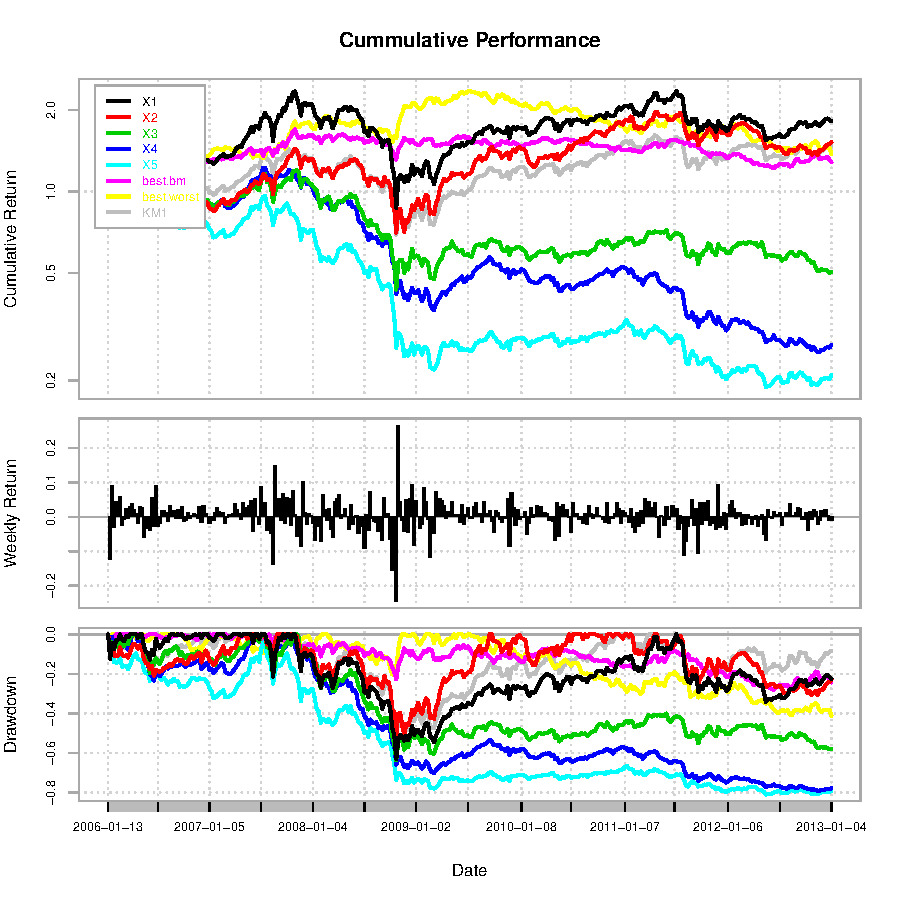
\includegraphics{graphics/plot-004}
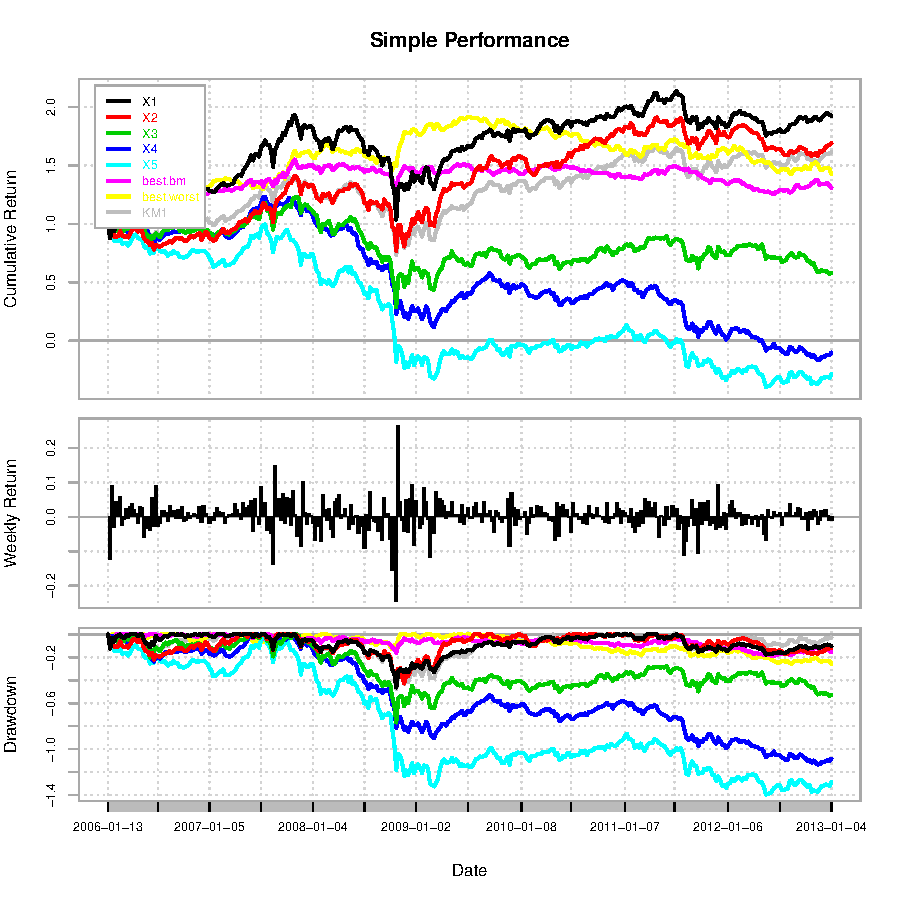
\includegraphics{graphics/plot-005}
\end{tabular}

%\end{landscape}
\subsection{Relative Returns}
\begin{tabular}{cc}
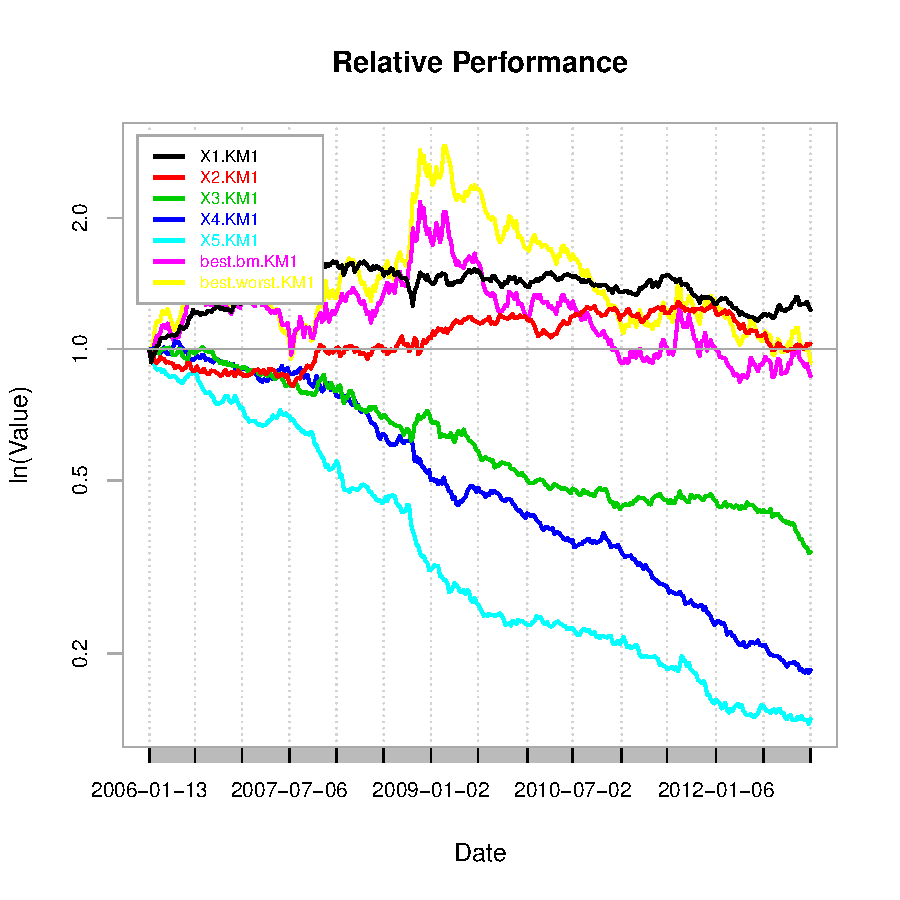
\includegraphics{graphics/plot-006}
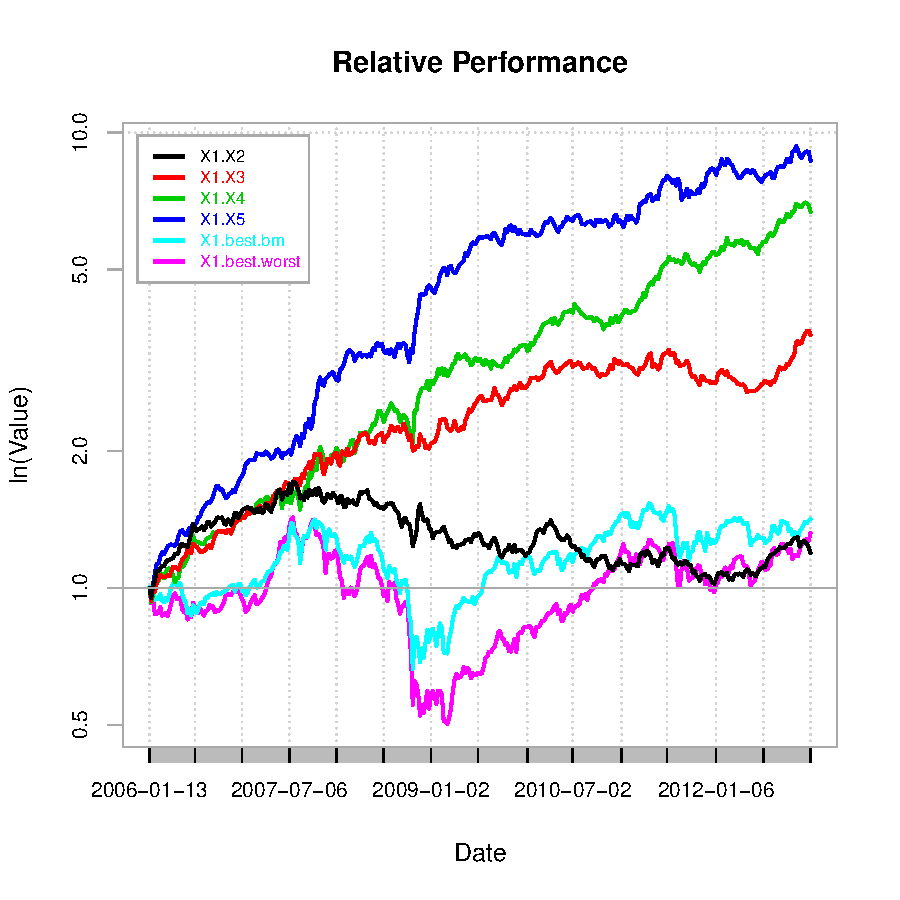
\includegraphics{graphics/plot-007}
\end{tabular}
\subsection{Other Charts}
\begin{tabular}{cc}
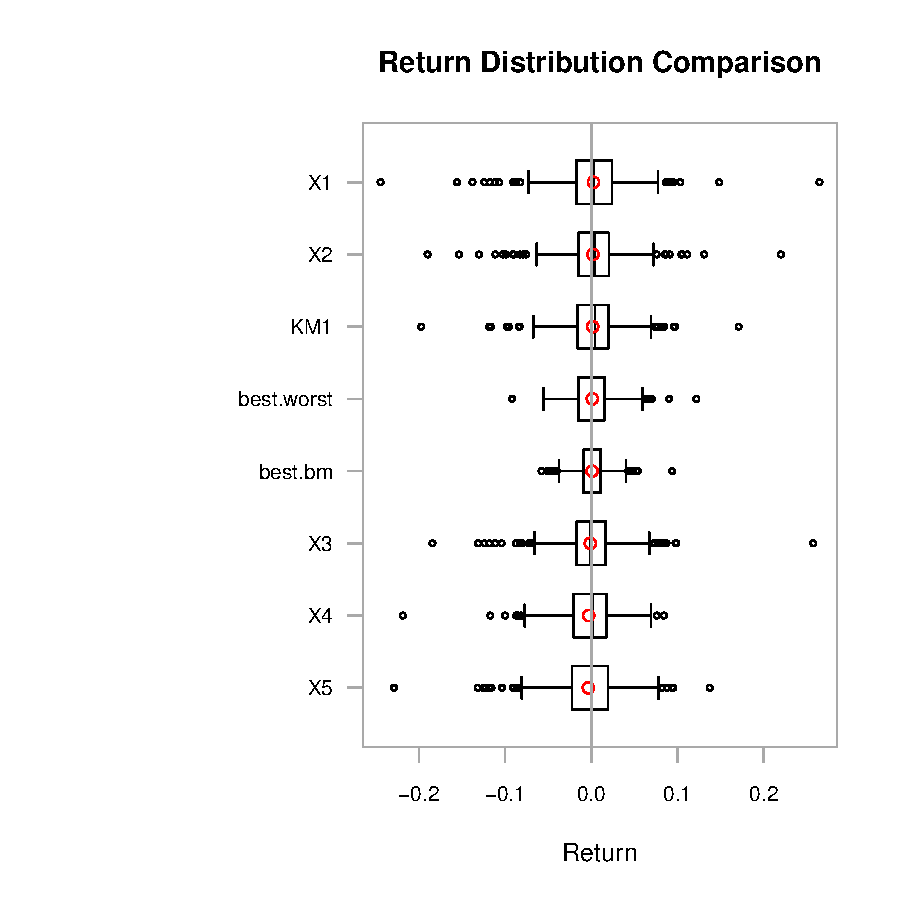
\includegraphics{graphics/plot-008}
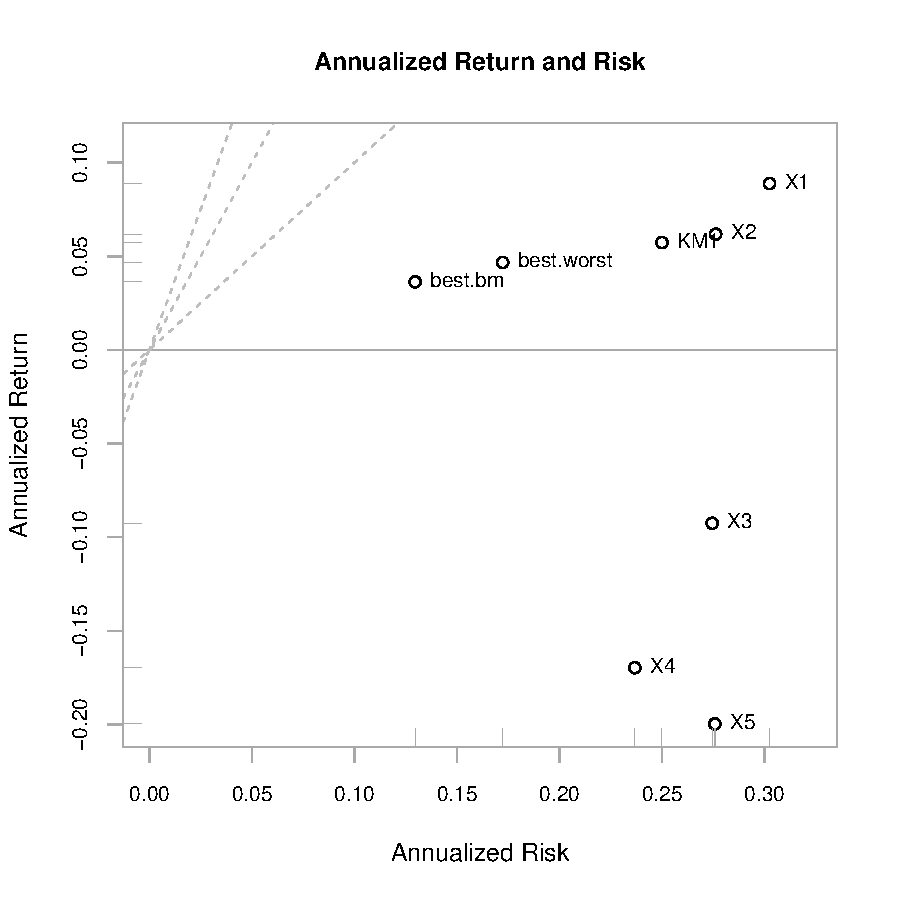
\includegraphics{graphics/plot-009}
\end{tabular}
\section{3yr Performance}
%\begin{landscape}
\subsection{Returns}
\begin{tabular}{cc}
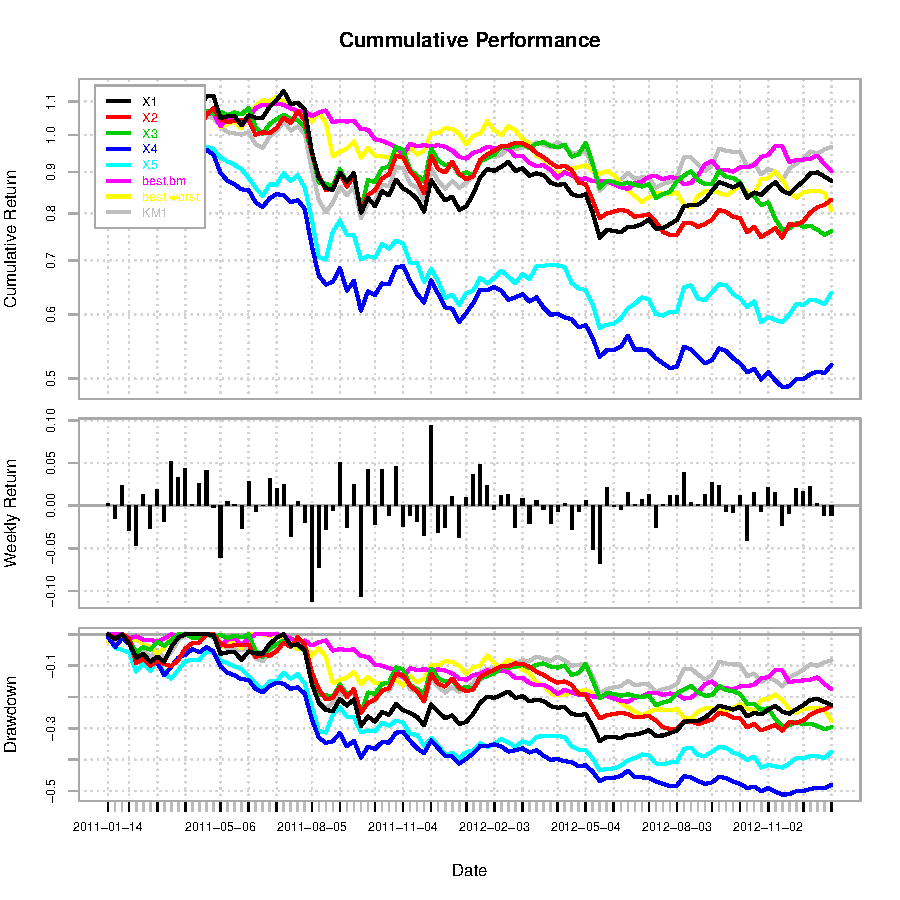
\includegraphics{graphics/plot-010}
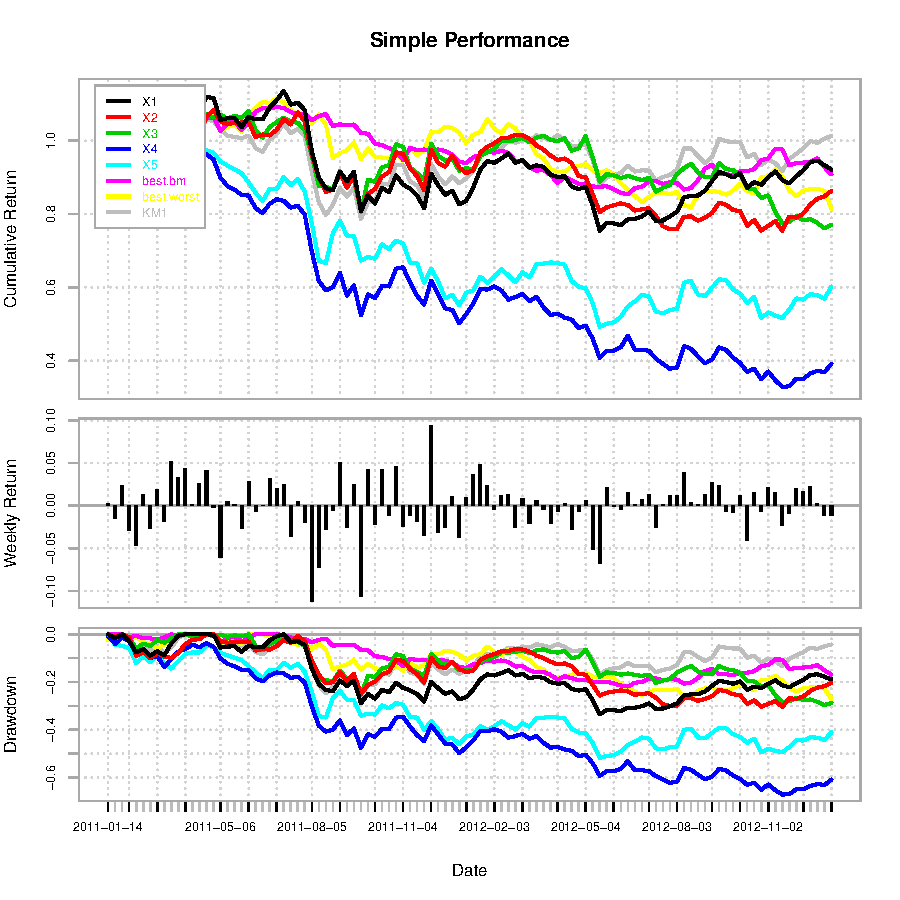
\includegraphics{graphics/plot-011}
\end{tabular}
%\end{landscape}
\subsection{Relative Returns}
\begin{tabular}{cc}
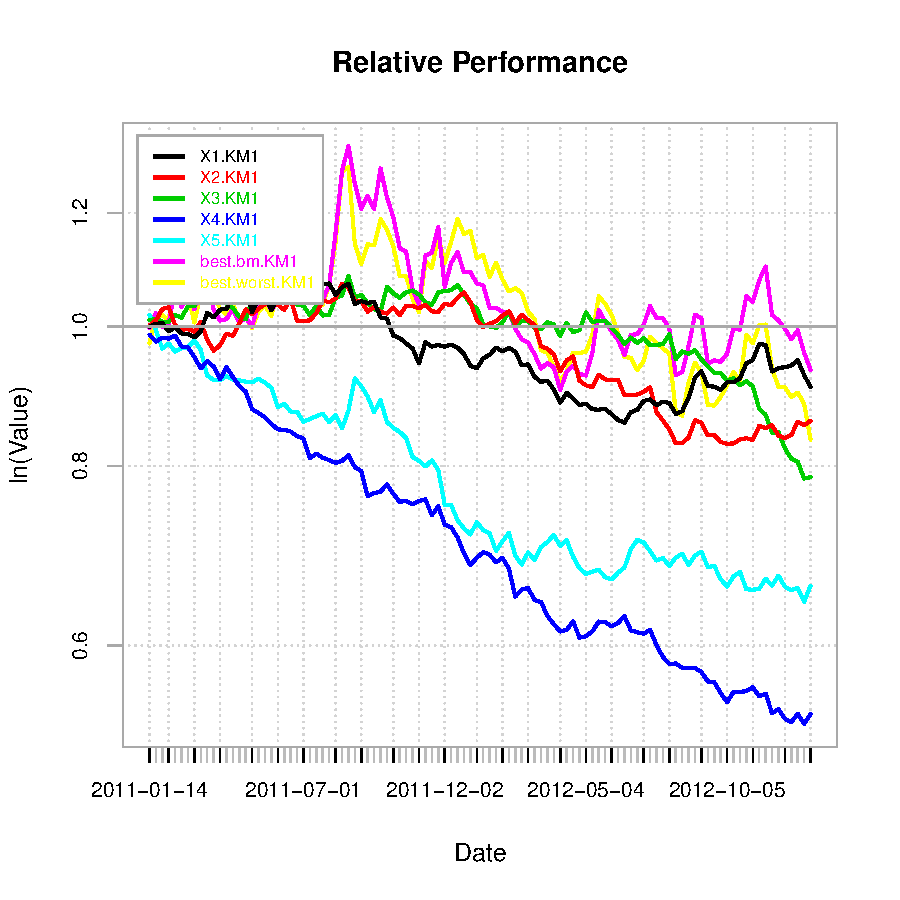
\includegraphics{graphics/plot-012}
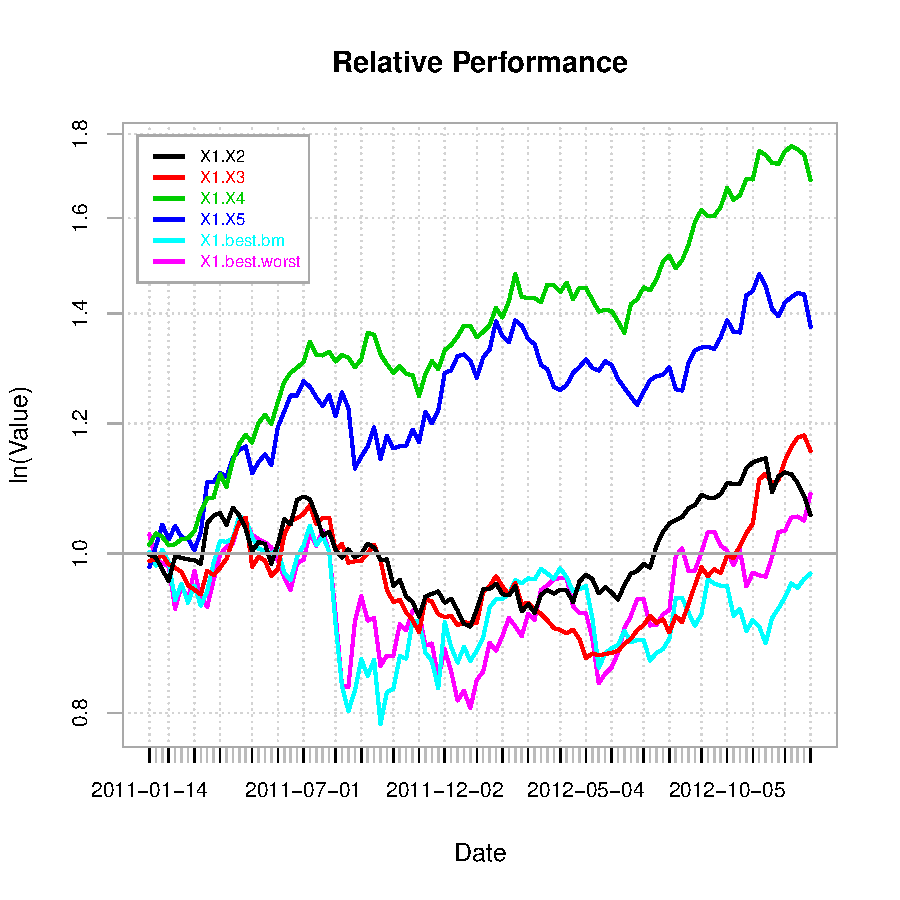
\includegraphics{graphics/plot-013}
\end{tabular}
\subsection{Other Charts}
\begin{tabular}{cc}
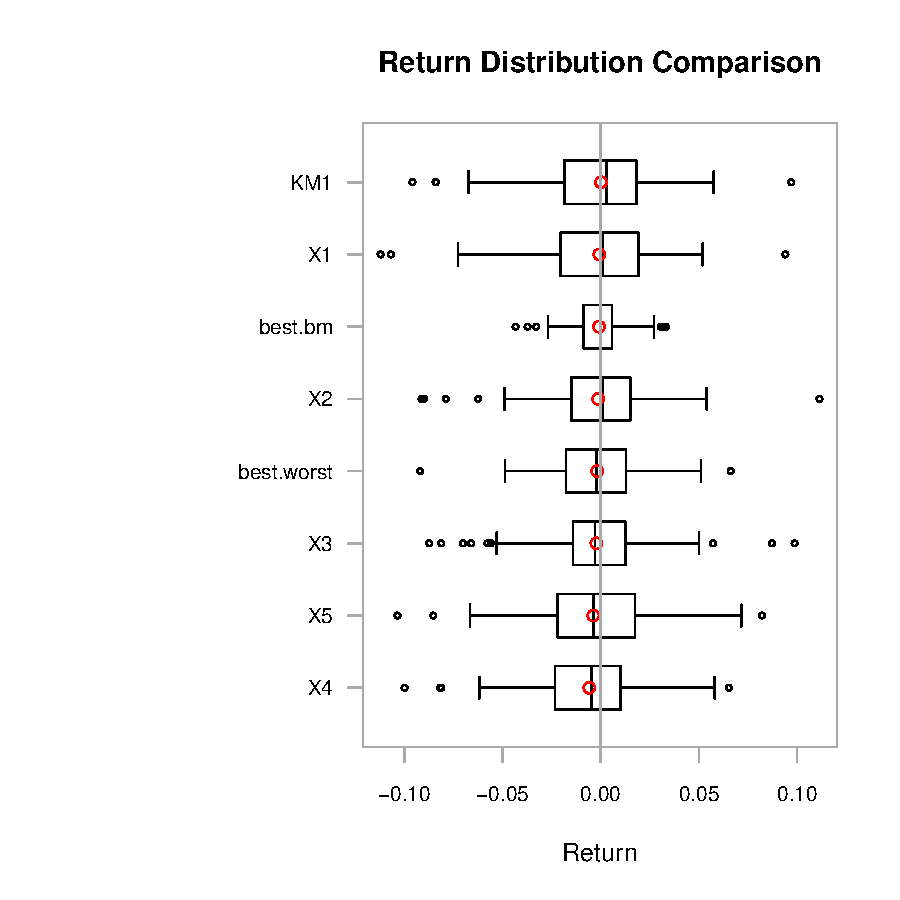
\includegraphics{graphics/plot-014}
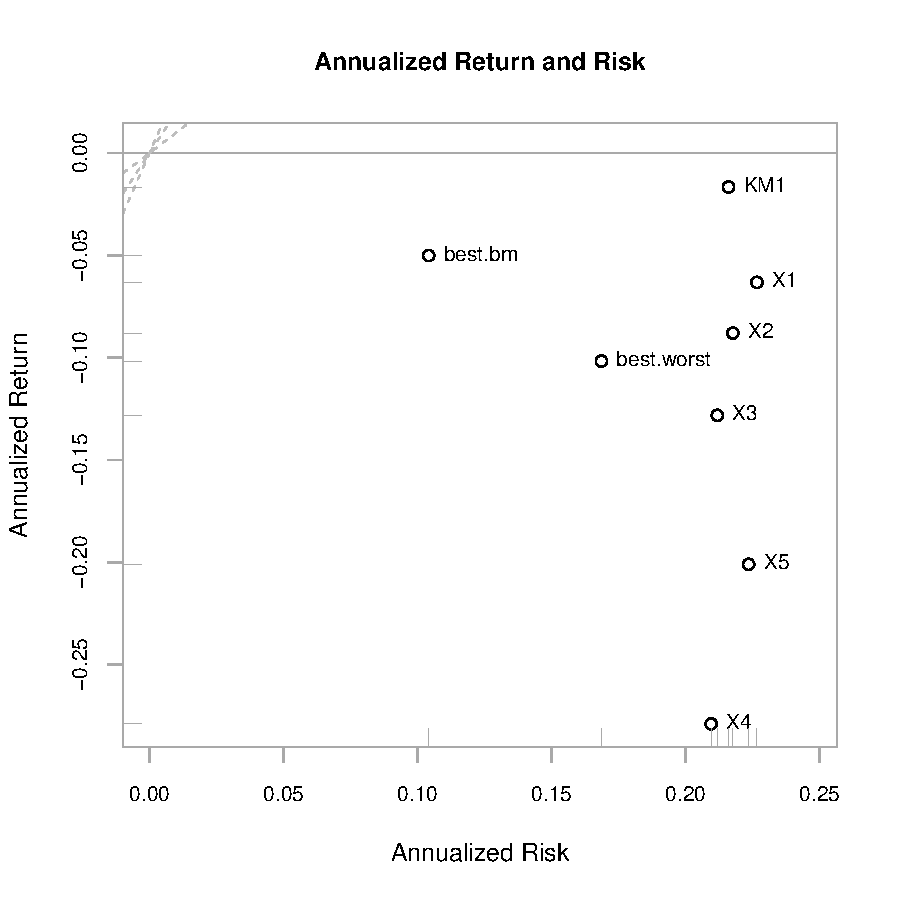
\includegraphics{graphics/plot-015}
\end{tabular}
\section{1yr Performance}
%\begin{landscape}
\subsection{Returns}
\begin{tabular}{cc}
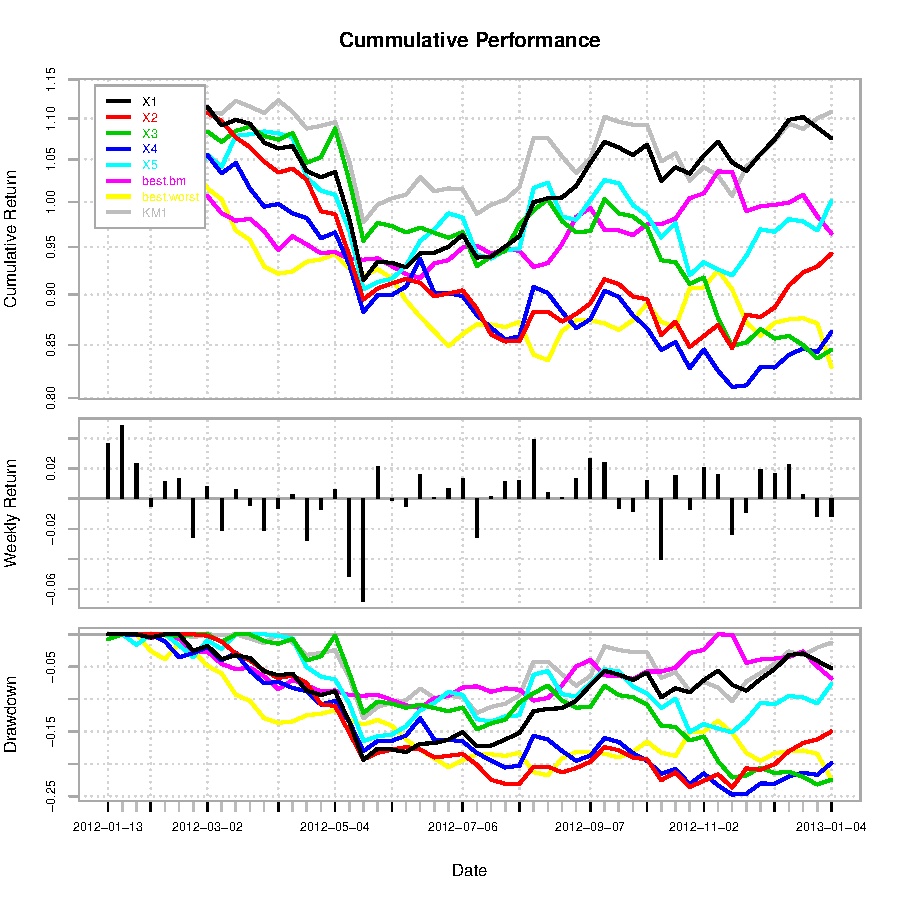
\includegraphics{graphics/plot-016}
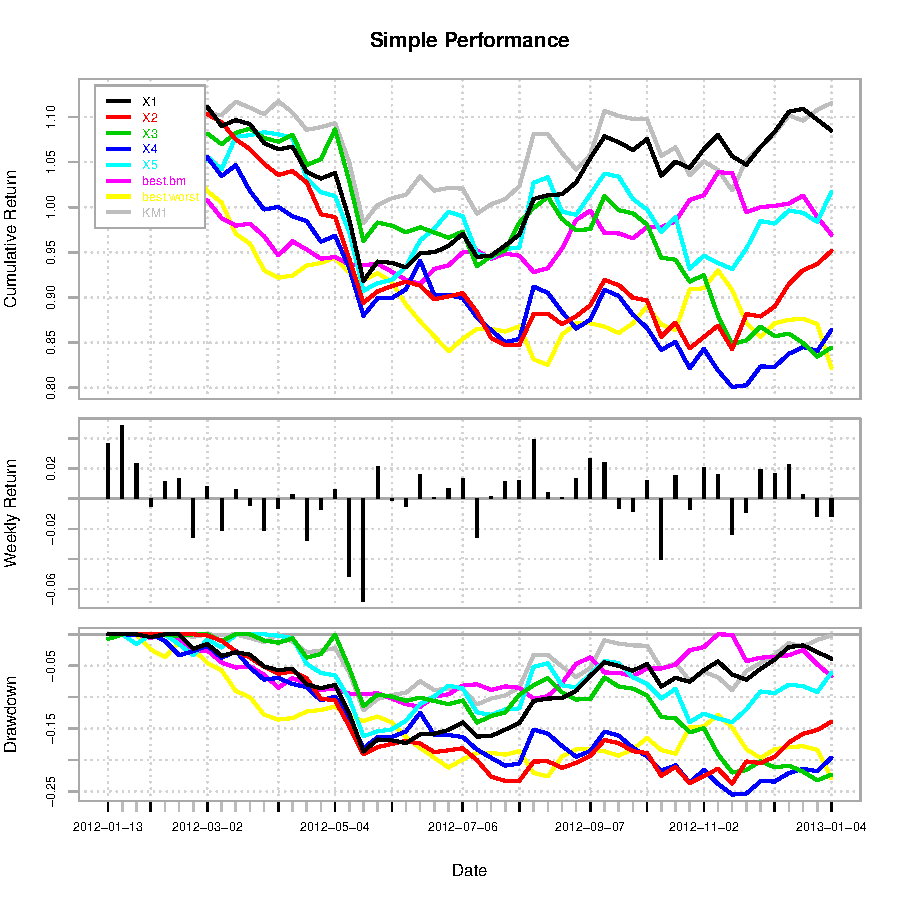
\includegraphics{graphics/plot-017}
\end{tabular}
%\end{landscape}
\subsection{Relative Returns}
\begin{tabular}{cc}
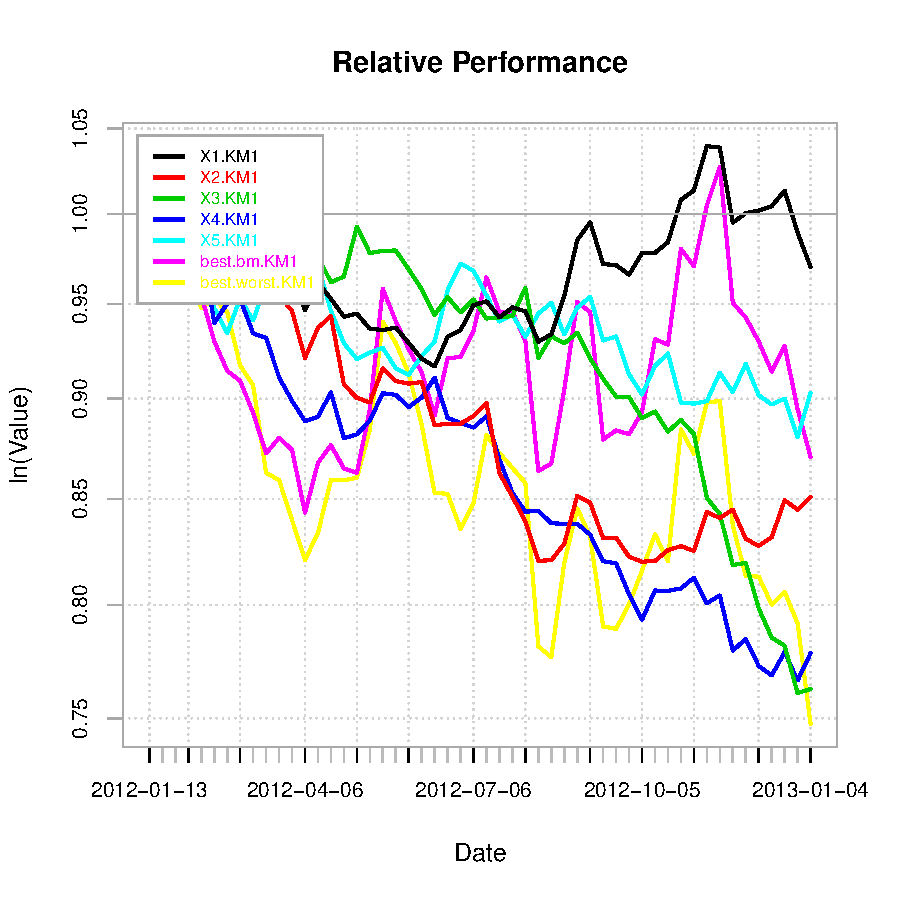
\includegraphics{graphics/plot-018}
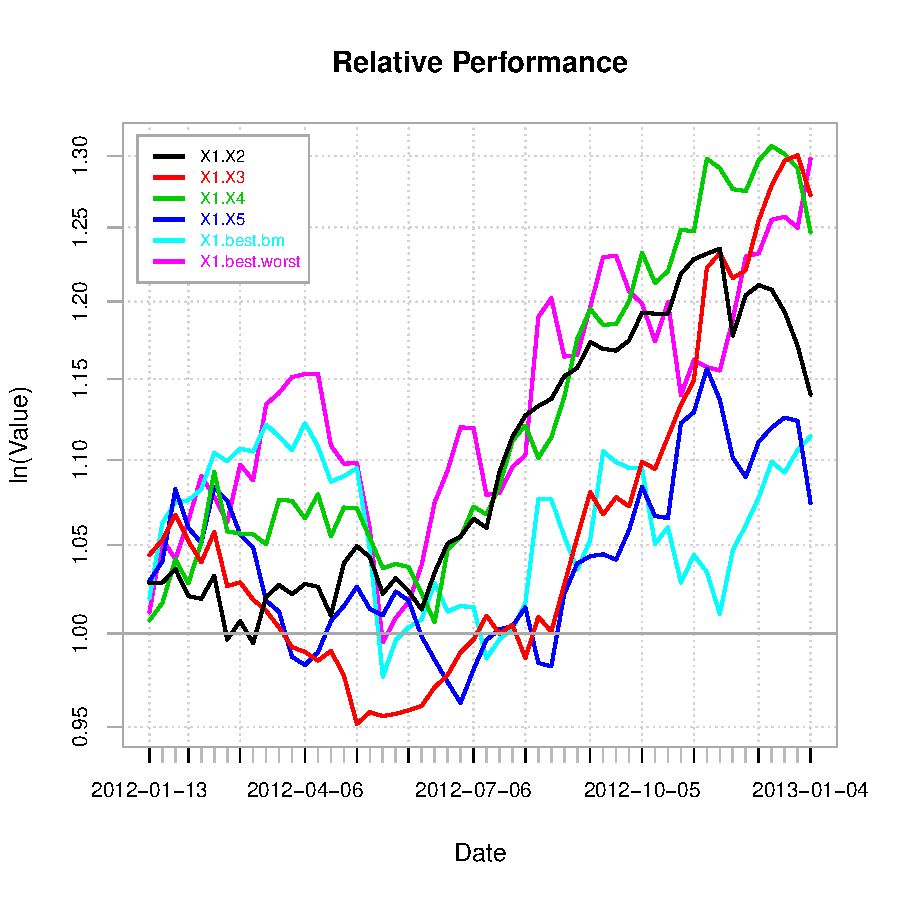
\includegraphics{graphics/plot-019}
\end{tabular}
\subsection{Other Charts}
\begin{tabular}{cc}
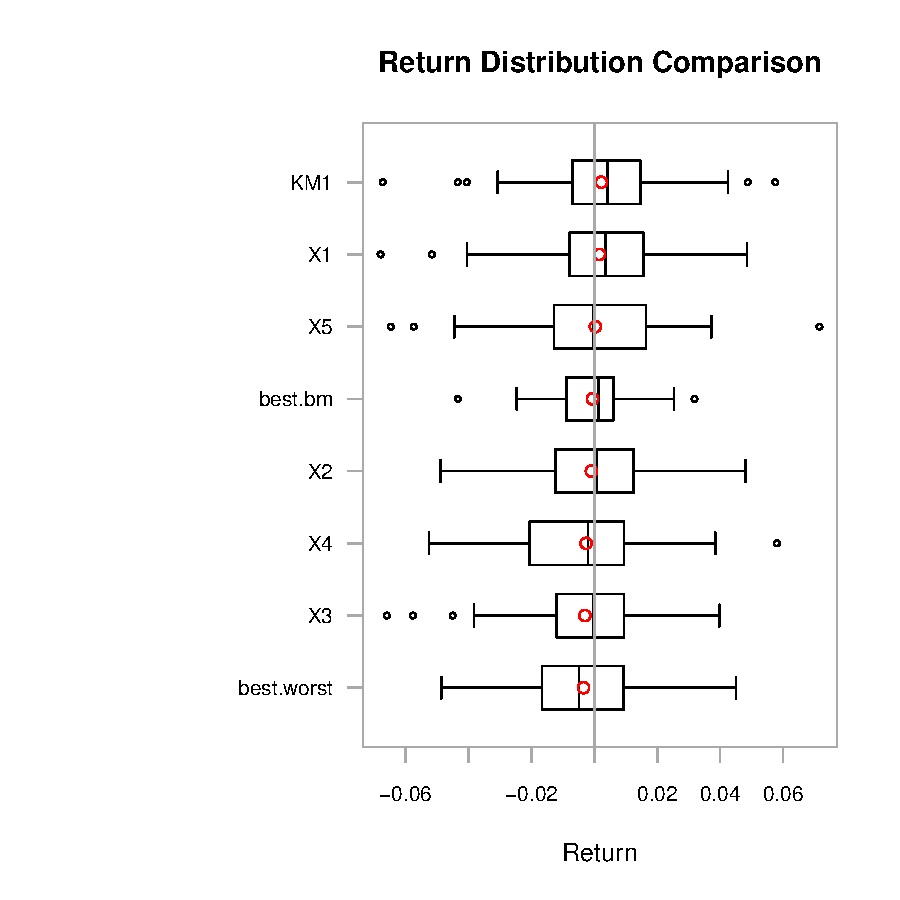
\includegraphics{graphics/plot-020}
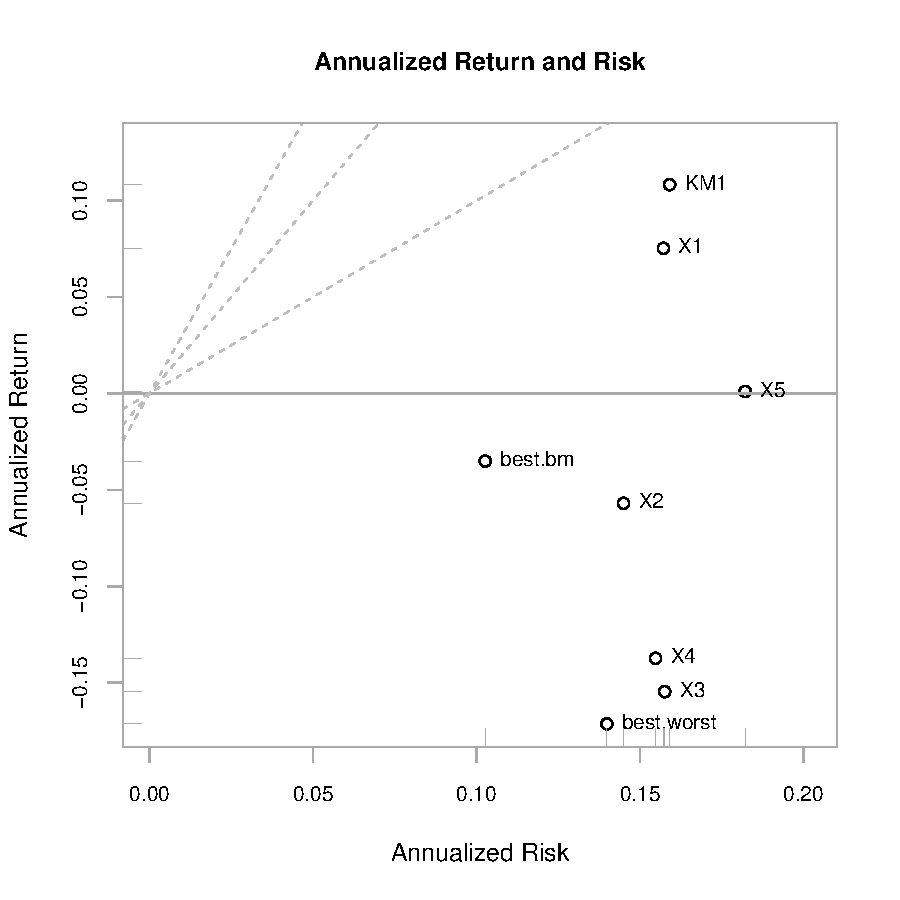
\includegraphics{graphics/plot-021}
\end{tabular}

\end{document}
